\documentclass[12pt]{article}

\usepackage[bottom = 15mm]{geometry}
\usepackage[utf8]{inputenc}
\usepackage[T2A]{fontenc}
\usepackage[russian]{babel}
\usepackage{graphicx}
\usepackage{caption}
\usepackage{amssymb, amsmath}
\usepackage{mathrsfs}

\textwidth = 16 cm
\textheight = 23  cm
\oddsidemargin = 0 pt
\topmargin = -1.5 cm
\parindent = 20 pt
\parskip = 0 pt
\flushbottom



\title{{\bf Задача 3.2.6\\ Исследование гальванометра}}
\author{Лось Денис (группа 611)}
\date{11 сентября 2017}




\begin{document}

\maketitle

\paragraph{Цель работы: } изучение работы высокочувствительного зеркального гальванометра магнитоэлектрической системы в режимах измерения постоянного тока и электрического заряда.

\paragraph{В работе используются: } зеркальный гальванометр с осветителем и шкалой, источник постоянного напряжения, делитель напряжения, магазин сопротивлений, эталонный конденсатор, вольтметр, переключатель, ключи, линейка.

\section*{Введение}
Баллистическим гальванометром называют электроизмерительный прибор магнитоэлектрической системы, отличающийся высокой чувствительностью к току  и сравнительно большим периодом колебаний подвижной системы(рамки)
\par
 	Главной частью баллистического гальванометра является подвешенная на вертикальной нити рамка, помещённая в поле постоянного магнита. Вырез цылиндрической формы в полюсах магнита и ферромагнитный циллиндр на оси системы делают поле в зазоре радиальным. Скреплённое с рамкой зеркальце служит для измерения угла поворота рамки. К рамке прикреплён полый цилиндр, который сильно увеличивает момент инерции и, следовательно, период колебаний подвижной системы, не очень её утяжеляя. Магнит и подвижная система заключены в защитный кожух. В баллистических нальванометрах применяют сильный постоянные магниты и рамки с большим количеством витков, подвешенные на тонких нитях с малой упругостью.
\par
	Баллистический гальванометр позволяет измерять как постоянный ток (стационарный режим), так и заряд, протекший через рамку за некоторое время (баллистический режим). В баллистическом режим гальванометр может работать, если время протекания заряда много меньше периода собственных колебаний подвижной рамки. Поэтому период колебаний рамки делают большим (5-15 с). 

\paragraph{Уравнение движения подвижной системы}
\par	
	На помещённую в магнитное поле рамку гальванометра действуют следующие моменты сил: момент закрученной нити, момент магнитных сил и тормозящий момент, зависящиий от сопротивления воздуха и от вихревых токов, вызывающих электромагнитное торможение. 
\par
	Механический момент $M_1$ упругих сил нити пропорционален углу поворота рамки:
\[
 	M_1 = -D \varphi,
\]	
где $D$ --- модуль кручения нити, а $\varphi$ --- угол поворота рамки от положения равновесия.
\par	
	Если рамка с числом витков $N$, обтекаемая током $I$, помещена в магнитное поле с индукцией $B$, то на боковые стороны рамки действуют силы, равные $lBNI$, где $l$ --- длина боковой стороны. Обозначив через $r$ расстояние от боковой стороны до оси вращения, найдём момент пары сил
\[
	M_2 = 2 r l B N I = B S N I,
\]	
где $S$ --- плошадь одного витка рамки.
\par
	Тормозящий момент складывается из моментов сил электромагнитного торможения и сил трения о воздух. В рамке, движущейся в магнитном поел с угловой скоростью $\dot\varphi$, наводится ЭДС индукции:
\[
	\mathscr{E}_\text{инд} = - \frac{d\Phi}{dt} = - BSNN\dot\varphi,
\]
где $\Phi$ --- магнитный поток, пронизиывающий рамку. Пренебрегая самоиндукцией рамки, можно считать, что эта ЭДС вызывает ток индукции $I_\text{инд} = -BSN\dot\varphi / R_\Sigma$. Здесь $R_\Sigma $ --- полное сопротивлений цепи, состоящее из сопротивления рамки $R_0$ и сопротивления внешнего участка цепи $R: R_\Sigma =  R_0 + R$. Тормозящий момент
\[
	M_3 = BSNI_\text{инд} = - \frac{\left(BSN\right)^2}{R_\Sigma} \dot\varphi
\]
\par
	В большинстве случаев данный момент существенной превосходит момент трения рамки воздух, которым, следовательно, можно пренебречь. Уравнение рамки принимает вид:
\[
	J \ddot \varphi = \Sigma M,
\]	
где $J$ --- момент инерции подвижной системы.
Объединяя все полученные уравнения можно получить:
\[
	J\ddot \varphi + \frac{\left(BSN\right)^2}{R_\Sigma} \dot \varphi + D \varphi = BSNI.
\]
Разделим обе части уравнения на $J$ и введём обозначения
\begin{equation*}
	\left.
	\begin{aligned}
		\frac{\left(BSN\right)^2}{JR_\Sigma} = 2 \gamma \\
	    \frac{D}{J} = \omega_0^2 \\
	    BSN / J = K
	\end{aligned}
	\right\}
\end{equation*}
Уравнение движение рамки примет вид
\begin{equation}
	\ddot \varphi + 2\gamma \dot \varphi + \omega_0^2\varphi = KI \label{osc}
\end{equation}
Следует отметить, что ток $I$ в уравнении определяется величиной ЭДС $\mathscr{E}$ внешнего источника, к которому подключён гальванометр $I = \mathscr{E} / R_\Sigma $, а влияние индукционного тока, тормозящего движение рамки, отражает слагамое, пропорциональное $\dot \varphi$.
\paragraph{Режим измерения постоянного тока}
\par 
	Если через рамку пропускать постоянный ток (достаточно долго, чтобы затухли колебания подвижной системы), то  в уравнении (\ref{osc}) можно положить $\ddot \varphi = \dot \varphi = 0$, тогда для угла поворота
\[
	\varphi = \frac{K}{\omega_0^2}I = \frac{BSN}{D}I = \frac{I}{C_I}.
\]
Величина $C_I$ называется {\bf динамической} постоянной гальванометра.
\[
	C_I = \frac{I}{\varphi} = \frac{D}{BSN}.
\]
\paragraph{Режим измерения заряда}
\par 
	Период свободных колебаний баллистического гальванометра благодаря искуственному увеличению момента инерции рамки оказывается очень большим (порядка десятка секунд). Если пропустить через рамку короткий импульс тока, то можно считать, что весь ток успевает пройти при неотклонённом положении рамки. Рамка, однако, при этом получает толчок, в результате которого возникает движение, описываемое уравнением свободных колебаний
\[
	\ddot \varphi + 2 \gamma \dot \varphi + \omega_0^2 \varphi = 0 \label{free_osc}
\]
при начальных условиях $\varphi = 0$, $\dot \varphi = \dot \varphi_0$ при $t = 0$.
\par
	Для вычисления скорости $\dot \varphi_0$, полученной в результате толчка, умножим уравнение (\ref{free_osc}) на $dt$ и проинтегрируем по времени от 0 до $\tau$, где $\tau$ --- момент окончание токового импульса:
\[
	\int\limits_0^\tau \ddot \varphi \,dt + 2\gamma \int\limits_0^\tau \dot \varphi \,dt + \omega_0^2 \int\limits_0^\tau \varphi \,dt = K \int\limits_0^\tau I \,dt
\]
Второе и третье слагаемые пренебрижимо малы:
\[
	2 \gamma \int\limits_0^\tau \dot \varphi \,dt \approx 0, \qquad \omega_0^2 \int\limits_0^\tau \varphi \, dt \approx 0 
\]
В результате мы имеем:
\[
	\dot \varphi(\tau) = K \int\limits_0^\tau I \,dt = Kq,
\]
где $q$ --- полный электрический заряд, прошедший через рамку за время импульса.
\par
	Таким образом, при пропускании коротких импульсов тока через баллистический гальванометр начальная скорость движения раамки пропорциональна полному электрическому заряду, прошедшему через рамку за всё время импульса. Также можно заметить, что наибольший угол, на который отклоняется рамка, также пропорционален $q$.
\par
	Величина $C_Q = q / \varphi_\text{max}$ называется {\bf баллистической} постоянной гальванометра. В отличие от динамической постоянной гальванометра, баллистическая постоянная существенно зависит от режима работа гальванометра(от сопротивления цепи).
\par
	Расчёт показывает, что максимальный отброс достигается при полном отсутствии затухания (тормозящий индукционный ток отсутствует при обрыве в цепи):
\[
	\varphi_\text{max св} = \frac{\dot \varphi(\tau)}{\omega_0} = \frac{Kq}{\omega_0}
\]
В этом случае, однако, возникшие в результате отброса колебания рамки не будут успокаиваться, и прибор не скоро может быть использован для повторных измерений.		
\par
	Обычно удобнее всего работать в режиме, близком к критическому. При этом обеспечивается быстрое затухание колебаний, и чувствительность прибора достаточно высока. В случае критического затухания
\[
	\varphi_\text{max кр} = \frac{Kq}{\omega_0 e}
\]		
Таким образом, в критическом режиме максимальное отклонение зайчика в $e$ раз меньше, чем в режиме свободных колебаний. Отсюда следует
\[
	\frac{C_\text{$Q_\text{кр}$}}{C_\text{$Q_\text{св}$}} = e
\]
\subsection*{Определение динамической постоянной}
\par
	Схема для исследования гальванометра в стационарном режиме представлена на рис.1
\begin{figure}[h!]
	\centering
	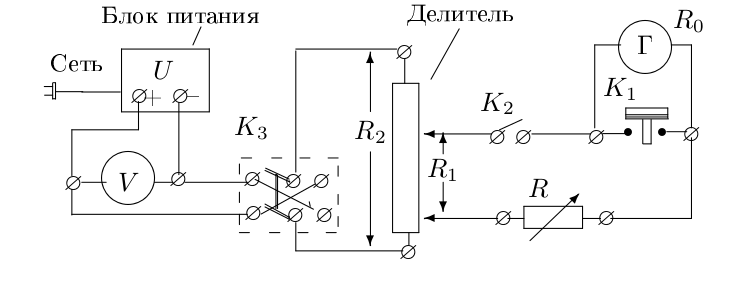
\includegraphics[width = 15cm, height = 6cm]{image1.png}
	\caption{Схема установки для работы гальванометра в стационарном режиме}
\end{figure}
\par			
При малых $R_1$ сила тока, протекающего через гальванометр может быть вычислена по формуле:
\[
	I = U_0\, \frac{R_1}{R_2}\, \frac{1}{R + R_0},
\]	
где $U_0$ --- показания вольтметра, $R_1 / R_2$ --- положение делителя, $R$ --- сопротивлени е магазина, $R_0$ --- внутреннее сопротивление гальванометра.
\par
	Угол отклонения рамки от положения равновесия измеряется с помощью осветителя, зеркальца, укреплённого на рамке, и шкалы, на которую отбрасывается луч света от зерькальца. Координата $x$ светового луча на шкале связана с углом отклонения рамки формулой
\[
	x = \alpha \tg(2\varphi),
\]	 
где $a$ --- расстояние от шкалы до зеркальца. При малых углах можно считать, что $\varphi = x / 2a$.
\par
Динамическая постояннная:
\[
	C_I = \frac{I}{\varphi} = \frac{2aI}{x}
\]
\subsection*{Определение критического сопротивления гальванометра}
\par
	Измерение критического сопротивления гальванометра также может быть выполено с помошью схемы, изображённой на рис.1.
\par
	При больших $R$ свободное движение рамки носит колебательный характер. С уменьшением $R$ затухание увеличивается, и колебательный режим переходим в апериодический.
\par
	Логарифмический декремент затухания $\Theta$:
\[
	\Theta = \ln \Delta = \gamma T = \ln \frac{x_n}{x_\text{n+1}}.
\]	
Измеряя зависимость логарифмического декремента затухания от сопротивления внешней цепи, можно найти $R_\text{кр}$, т.е значение $R$, при котором $\Theta \to \infty $. Измерения логарифмического декремента при сильном затухании затруднены, поэтому исследуем зависимость $\Theta$ от $R$. Получим, что
\[
	\Theta = \gamma T = 2 \pi \frac{\gamma}{\omega} = \frac{2 \pi \gamma}{\sqrt{\omega_0^2 - \gamma^2}} = \frac{2 \pi R_3}{\sqrt{\left(R_0 + R_3\right)^2 - R_3^2}}
\]				
где $R_3 = \frac{\left(BSN\right)^2}{2\sqrt{JD}} = R_0 + R_\text{кр}$.
\par 		
Из этого получим, что
\[
	\frac{1}{\Theta^2} = \frac{\left(R_0 + R\right)^2}{4 \pi^2 R_3^2} - \frac{1}{4\pi^2}
\]		 
\par
	Последнее уравнение, представленное на графике в координатах $X = \left(R_0 + R\right)^2, Y = 1 / \Theta^2$, имеет вид прямой, угол наклона которой позволяет рассчитать критическое сопротивление:
\[
	R_\text{кр} = \frac{1}{2 \pi} \sqrt{\frac{\Delta X}{\Delta Y}} - R_0 
\]
\newpage	 
\subsection*{Определение баллистической постоянной и критического сопротивления гальванометра, работающего в баллистическом режиме}
\par
	Для изучения работы гальванометра в режиме измерения заряда используется схема, представленная на рис.2
\begin{figure}[h!]
	\centering
	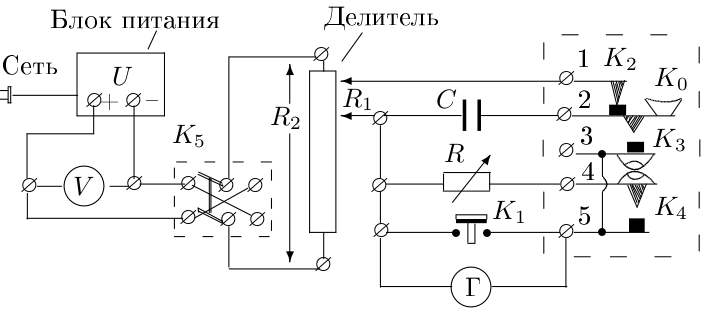
\includegraphics[width = 15cm, height = 6cm]{image2.png}
	\caption{Схема установки для определения баллистической постоянной}
\end{figure}	 	 
\par
	Система ключей устроена так, что нормально ключ $K_2$ замкнут, а ключи $K_3$ и $K_4$ разомкнуты. При нажатии на кнопку $K_0$ сначала размыкается ключ $K_2$, затем размыкается ключ $K_3$ и через некоторое время --- $K_4$.
\par	
	При нормальном положении кнопки $K_0$ конденсатор $C$ заряжается до напряжения
\[
	U_C = \frac{R_1}{R_2}\,U_0.	
\]	 
Заряд конденсатора равен
\[
	q = CU_C = \frac{R_1}{R_2}\, U_0 C.
\]
\par
	При нажатии на кнопку $K_0$ конденсатор отключается от источника постоянного напряжения и подключается к гальванометру.
\par	
	Первый отброс зацчика $l_\text{max}$ после нажатия на кнопку $K_0$ зависит от сопротивления внешней цепи, подключённой к гальванометру. Для определения $R_\text{кр}$ испольуется то обстоятельство, что в критическом режиме максимальное отклонение зайчика в $e$ раз меньше, чем у гальванометра без затухания.
\par
	Величину максимального отклонения гальванометра без затухания $\varphi_0$ можно рассчитать, если при разомкнутой цепи измерены максимальное отклонение рамки $\varphi_1$ и логарифмический декремент затухания $\Theta_0$. При $\gamma \ll \omega_0$
\[
	\varphi_0 = \varphi_1 \cdot e^{\Theta_0 / 4}
\]	 
Баллистическая постоянная гальванометра $C_\text{$Q_\text{кр}$}$ определяется при критическом сопротивлении $\left(R = R_\text{кр}\right)$:
\[
	C_\text{$Q_\text{кр}$} = \frac{q}{\varphi_\text{max кр}} = 2\alpha\,\frac{R_1}{R_2}\,\frac{U_0 C}{l_\text{max кр}}
\]
где $l_\text{max кр}$ --- величина первого отброса в критическом режиме(мм), $a$ --- расстояние от зеркальца до шкалы(м), а $U_0 C$ --- заряд, выраженный в кулонах.
\section*{Ход работы}
\paragraph{Определение критического сопротивления}
\begin{enumerate}
	\item
		Соберём схему согласно рис.1 и установим такое значение $R$, при которым зайчик бы отклонялся почти на всю шкалу. Разомкнём ключ $K_2$ и измерим два последовательных отклонения зайчика в одну сторону для расчёта логарифмического декремента затухания разомкнутого гальванометра $\Theta_0 = 0.11$. Период свободных колебаний рамки $T_0 \approx 5 \text{c}$
	\item
		Подберём наибольшее сопротивление магазина $R$, при котором при размыкании ключа $R_3$, зайчик не переходит за нулевое значение, которое достаточно близко к критическому сопротивлению цепи $R_\text{кр}$. В данном случае $R \approx R_\text{кр} \approx 8990$ Ом.
	\item
		В интервале от $3 R_\text{кр}$ до $10 R_\text{кр}$ будем измерять два последовательных отклонения зайчика в одну сторону после размыкания ключа $K_3$, чтобы рассчитать логарифмический декремент затухания $\Theta$.
		\begin{table}[h!]
			\centering
			\begin{tabular}{|c|c|c|c|c|c|}
			\hline
			$R$, Ом & $x_n$,мм & $x_\text{n+1}$, мм & $\Theta$ & $\Delta_\Theta$ & $\sigma_\Theta \cdot \%$ \\
			\hline
			35960 & 104 & 37 & 1.146 & 0.004 & 0.3  \\
			\hline
			44950 & 95 & 39 & 0.890 & 0.005 & 0.6\\
			\hline
			53940 & 88 & 41 & 0.764 & 0.006 & 0.8\\
			\hline
			62930 & 79 & 41 & 0.656 & 0.007 & 1.1\\
			\hline
			71920 & 78 & 42 & 0.619 & 0.008 & 1.3\\
			\hline
			80910 & 70 & 40 & 0.560 & 0.009 & 1.6\\
			\hline
			89900 & 67 & 41 & 0.491 & 0.011 & 2.2\\
			\hline
			\end{tabular}
		\end{table}
	\item
		Построим график $1/\Theta^2 = f((R + R_0)^2)$, где $R_0 = 500$ Ом --- внутреннее сопротивление гальванометра, в координатах $Y = 1 / \Theta^2$ и $X = (R + R_0)^2$ и по наклону прямой рассчитаем критическое сопротивление цепи $R_\text{кр}$
		\[
	R_\text{кр} = \frac{1}{2 \pi} \sqrt{\frac{\Delta X}{\Delta Y}} - R_0 
\]
		\newpage	
		\begin{table}[h!]
			\centering
			\begin{tabular}{|c|c|c|}			
			\hline
			$X$, ${\text{кОм}}^2$ & $Y$ & $\Delta_Y$ \\
			\hline
			1329.3 & 0.761 &  0.003 \\
			\hline
			2065.7 & 1.262 & 0.011 \\
			\hline 
			2963.7 & 1.713 & 0.019 \\
			\hline
			4023.4 & 2.324 & 0.036 \\
			\hline
			5244.7 & 2.610 & 0.048 \\			
			\hline 
			6627.6 & 3.189 & 0.072 \\
			\hline
			8172.2 & 4.148 & 0.129 \\			
			\hline			
			\end{tabular}
		\end{table}
		\begin{figure}[h!]
			\centering
			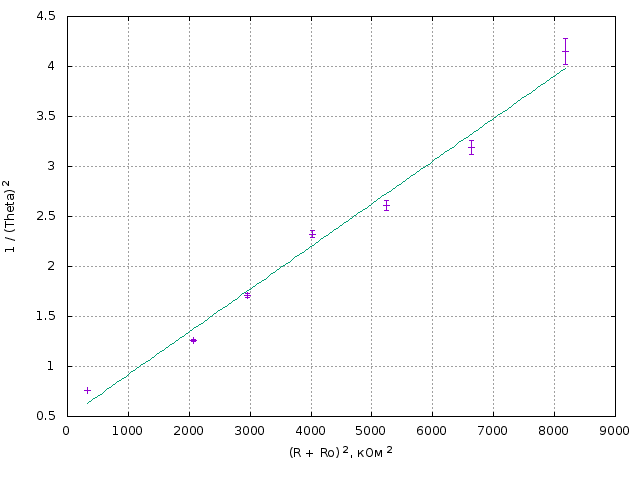
\includegraphics[width = 15cm, height = 8cm]{plot1.png}
			\caption{График зависимости $1 / \Theta^2$ от $(R + R_0)^2$}
		\end{figure}
	\par
		Методом наименьших квадратов находим, что
		\[
			\frac{\Delta Y}{\Delta X} = \left(42.67 \pm 2.18 \right) \cdot 10^{-5} \, {\text{кОм}}^2
		\]
	Следовательно, для $R_\text{кр}$ получаем, что
	    \[
	    	R_\text{кр} = \left(7204 \pm 180 \right) \/ \text{Ом}
	    \]			
\end{enumerate}
\paragraph{Баллистический режим}
\begin{enumerate}
	\item
		Соберём схему согласно рис.2 и установим сопротивление $R = 50$ кОм. Для измерения первого отброса зайчика в режиме свободных колебаний $\left(R = \infty\right)$ разомкнём цепь $R$, отсоединив одну из клемм магазина. Подберём делитель так, чтобы при замыкании ключа $K_0$ первый отброс $l_\text{max}$ соответствовал отклонению зайчика почти на всю шкалу.
\[
	l_\text{max св} = \left(21.7 \pm 0.1\right) \, \text{см}
\]
	\item
		Вновь подключим магазин $R$ и, не меняя положения делителя, снимем зависимость первого отброса от величины $R$.
		\newpage		
		\begin{table}[h!]
			\centering
			\begin{tabular}{|c|c|c|}
			\hline
			$R$, Ом & $1 / (R_0 + R) \cdot 10^{-5}$, $\text{Ом}^{-1}$ & $l_\text{max}$, см \\
			\hline
			40000 & 2.47 & 16.6\\
			\hline
			35000 & 2.82 & 16.4\\
			\hline
			30000 & 3.28 & 16.3\\
			\hline
			25000 & 3.92 & 15.5\\
			\hline
			20000 & 4.88 & 14.9\\
			\hline
			15000 & 6.45 & 13.1\\
			\hline
			10000 & 9.52 & 10.4\\
			\hline
			9000 & 10.53 & 9.9\\
			\hline
			8000 & 11.76 & 8.5\\
			\hline
			7000 & 13.33 & 7.3\\
            \hline
            6000 & 15.38 & 5.6\\		
			\hline
			\end{tabular}
		\end{table}
	\par
		В критическом режиме первый отброс в $e$ раз меньше, чем в режиме свободных колебаний. Поэтому будем уменьшать $R$ до тех пор, пока первый отброс не уменьшится до $1/3 - 1/4$ от максимальной величины.
	\par
		Положение делителя $R_1 / R_2 = 1 / 30$, ёмкость конденсатора $C = 2$ мкФ, расстояние от шкалы до зеркальца гальванометра $a = \left(132.0 \pm 0.5\right)$ см, тогда как $U_0 = 1.38$ В. 		
	\par
		Следовательно, баллистическая постоянная гальванометра 
\[
    C_\text{$Q_\text{кр}$} = 2a\, \frac{R_1}{R_2}\,\frac{U_0 C}{l_\text{max кр}}
\]	
\[
	C_\text{$Q_\text{кр}$} = \left(1.64 \pm 0.02 \right) \cdot 10^{-9}\, \frac{\text{Кл} \cdot\text{м}}{\text{мм}}
\]
	\item
		Время релаксации $t = R_0 C = 10^{-3}\, \text{с} \ll T_0 = 5 \, \text{с}$.
	\item
		Построим график $l_\text{max} = f[1 / \left(R_0 + R \right)]$ (рис.4), т.е. $x = 1 / \left(R_0 + R\right)\, \text{Ом}^{-1}$, и определим по нему критическое сопротивление гальванометра.
	\par
		Из графика получим, что $l_\text{max} = ax + b$, где
		\[
			a = - \left(87293 \pm 1234 \right) \, \text{Ом $\cdot$ см} \qquad b = \left(18.92 \pm 0.11 \right) \, \text{см},
	    \]
	    Отсюда находим, что
	    \[
	    	R_\text{кр} = R(l_\text{max} / e = 8 \text{см}) = \left(7494 \pm 114\right) \, \text{Ом}
	    \]
	    \begin{figure}[h!]
	    	\centering
	    	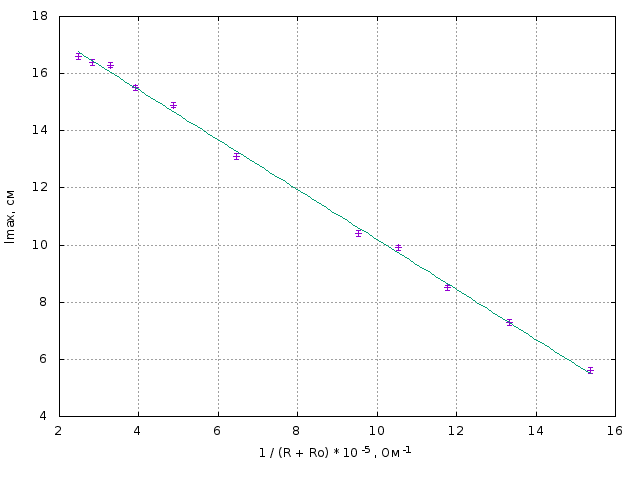
\includegraphics[width = 15cm, height = 7cm]{plot2.png}
	    	\caption{График зависимости $l_\text{max}$ от $1 / \left(R_0 + R\right)$}
	    \end{figure}	 		 
\end{enumerate}
\newpage
\paragraph{Определение динамической постоянной}
\begin{enumerate}
	\item
		Для выполнения данной части задачи специально была написана программа DyConstGalvanometer, моделирующая выполнение эксперимента. Демонстрация данной программы является частью отчёта.
	\item
		Снимем зависимость отклонения зайчика $x$ от сопротивления магазина $R$, измененяя сопротивление магазина, но не меняя делителя. Для данной виртуальной установки:
		\begin{align*}
			2a &= 2.64 \, \text{м} \\
			R_0 &= 500 \, \text{Ом}
		\end{align*}
		
	\item
		При  малых $R_1$ сила тока через гальванометр может вычислена как
		\[
			I = U_0 \, \frac{R_1}{R_2}\,\frac{1}{R_0 + R},
		\]
		а при малых углах отклонения, можно считать, что $\varphi = x / 2a$.
	\item
		Построим график $I = f(x)$ и по наклону прямой рассчитаем динамическую постоянную $C_I$:
		\[
			C_I = 2a\, \frac{\Delta I}{\Delta x}
		\]
		Положение делителя $R_1 / R_2 = 1 / 5000$, напряжение $U_0 = 1.41$ В.
        \newpage		
		\begin{table}[h!]
			\centering
			\begin{tabular}{|c|c|c|}
			\hline
			$R$, Ом & $I$, нА & $x$, мм \\
			\hline
			20000 & 13.657 & 45 \\
			\hline
			25000 & 11.059 & 36 \\
			\hline
			28000 & 9.895 & 32 \\
			\hline
			31000 & 8.952 & 29 \\
			\hline
			34000 & 8.174 & 26 \\
			\hline
			37000 & 7.520 & 24 \\
			\hline
            40000 & 6.963 & 22 \\
            \hline
            43000 & 6.483 & 21 \\			
			\hline
			\end{tabular}
		\end{table}				
		\begin{figure}[h!]
			\centering
			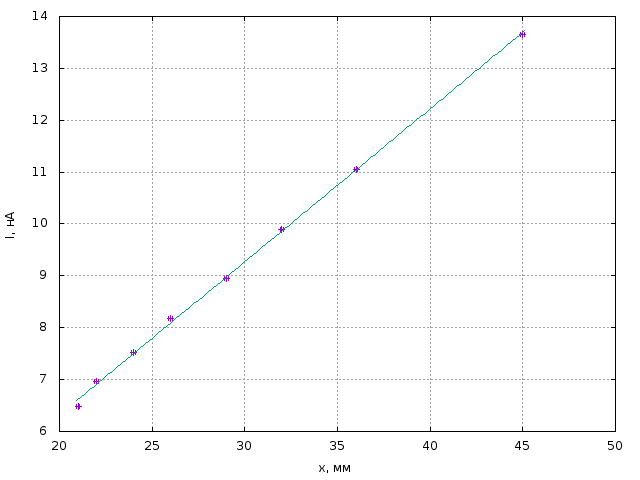
\includegraphics[width = 15cm, height = 8cm]{plot3.png}
			\caption{График зависимости $I = f(x)$}
		\end{figure}
	    Из графика
	    \[
	    	\frac{\Delta I}{\Delta x} = \left(0.295 \pm 0.004\right) \, \frac{\text{нА}}{\text{мм}}
	    \]
	    Следовательно, 
	    \[
	    	C_I = \left(0.78 \pm 0.01 \right) \, \frac{\text{нА} \cdot \text{м}}{\text{мм}}
	    \]				
\end{enumerate}

\end{document}